\documentclass[twocolumn]{article}
\usepackage[english]{babel}
\usepackage[utf8]{inputenc}
\usepackage{amsmath,amssymb,physics,mathtools,blindtext,graphicx,float}
\usepackage[a4paper,total={7.5in,10in}]{geometry}
\usepackage[labelfont=bf]{caption}

\begin{document}
\begin{large}

\section*{TOV}
\begin{normalsize}
\textit{Abstract:} 
\end{normalsize}
\subsection*{Introduction}

After a star has exhausted its fuel it starts to collapse since there is not enough radiation pressure to counteract its own gravity. When the star has reached a certain density however, the electron degeneracy pressure becomes large enough to counteract the gravitational force and the star becomes a so called white dwarf. However, there is a limit to how much the electron degeneracy pressure can hold and if the mass of the star is larger than the Chandrasekhar limit $1.4$ M$_\odot$, it collapses further into either a neutron star, in which case the neutron degeneracy pressure counteracts gravity, or into a black hole. 

Assuming a spherically symmetric star, the newtonian equations for balance between the gravitational force and the pressure are given by
\begin{equation}
    \label{28maj1900}
    \begin{split}
        &\frac{\text{d}P}{\text{d}r} = -\frac{GM(r)\rho(r)}{r^2} \\ 
        &\frac{\text{d}M}{\text{d}r} = 4\pi r^2\rho(r)
    \end{split}
\end{equation}
where $P(r)$ is the pressure, $M(r)$ is the mass inside radius $r$, $\rho(r)$ is the density and $G$ is the gravitational constant. For a given pressure at the center $P(0)$ and density function $\rho(r)$ these equations can be integrated to give the radius of the star $R$ where $P(R)=0$ and the mass of the star which is given by $M(R)$. For very dense objects however, such as neutron stars, relativistic corrections to the equations above become important. These corrections are given in the so called Tolman-Oppenheimer-Volkoff (TOV) equations. In this report the mass and radii of white dwarfs and neutron stars are investigated using the TOV-equations by assuming a degenerate gas of electrons for the white dwarfs, and a degenerate gas of neutrons for the neutron stars.

\subsection*{Tolman-Oppenheimer-Volkoff equations}
The TOV-equations are solutions to Einstein's field equation inside a static spherically symmetric mass distribution. They are given by the following equations:
\begin{equation}
    \begin{split}
        &\frac{\text{d}P}{\text{d}r} = -\frac{G\left[P+\mathcal{E}\right]\left[M(r)+4\pi r^3P/c^2\right]}{c^2r^2[1-2GM(r)/(c^2r)]} \\ 
        &\frac{\text{d}M}{\text{d}r} = 4\pi r^2\frac{\mathcal{E}}{c^2}
    \end{split}
\end{equation}
where $\mathcal{E} = \rho c^2$ is the energy density and $c$ is the vacuum speed of light. Notice that the equation for the mass $M$ is the same as in the newtonian equations given in \eqref{28maj1900} but the equation for pressure is non-linear because pressure is itself a source of gravity in general relativity which makes the equation more complicated.

A comparison of these equations to the newtonian equations can be more readily made by multiplying the first equation by $4\pi r^2\mathcal{E}\text{d}r/c^2 = \text{d}M$ and cancelling $\mathcal{E}$ on both sides:
\begin{equation}
    \label{28maj1039}
    \begin{split}
        4\pi r^2\text{d}P &= -\frac{GM\text{d}M}{r^2}\left(1+\frac{P}{\mathcal{E}(r)}\right)\left(1+\frac{4\pi r^3P}{Mc^2}\right) \\ 
        &\hspace{2cm}\times\left(1-\frac{2GM}{c^2r^2}\right)^{-1}
    \end{split}
\end{equation}
The term on the left hand side is the force exerted on a infinitesimal shell between radii $r$ and $r+\text{d}r$. The first factor on the right hand side is the newtonian gravitational force from the interior acting on this shell. The other three factors are relativistic corrections which become important for dense and more massive stars. These factors all exceed unity which makes the gravitational force stronger and compresses the matter more compared to the newtonian case.

The TOV-equations can be integrated after an equation of state has been specified, $\mathcal{E}(P)$, which relates the energy density to the pressure. These will now be derived from Fermi statistics for a degenerate electron gas, corresponding to white dwarfs, and degenerate neutron gas, corresponding to neutron stars.

\subsection*{Equation of state}
\subsubsection*{\textit{Equation of state for a white dwarf:}}
In this model for a white dwarf, it is assumed that its matter content is composed of inert heavy nuclei (e.g. oxygen or carbon nuclei) in a sea of electrons. Due to the high density, the electrons are not bound to the nuclei and can move freely. Furthermore, it is assumed that the electrons form a zero temperature Fermi gas. From Fermi statistics, the number density of electrons is then given by
\begin{equation}
    \label{28maj0858}
    n = \frac{p_F^3}{3\pi^2\hbar^3}
\end{equation}
where $p_F$ is the Fermi momentum. The energy density is also given by 
\begin{equation}
    \mathcal{E}_e = 2\int\limits_0^{p_F}\sqrt{c^2p^2+m_e^2c^4}\frac{4\pi p^2}{(2\pi\hbar)^3}\text{d}p
\end{equation}
where $\sqrt{c^2p^2+m_e^2c^4}$ is the energy of an electron with momentum $p$ and mass $m_e$. By calculating this integral, one finds that 
\begin{equation}
    \label{28maj0910}
    \begin{split}
        &\mathcal{E}_e = \frac{(m_ec^2)^4}{8\pi^2(\hbar c)^3}\bigg[x_F\sqrt{1+x_F^2}\left(1+2x_F^2\right) \\ 
        &\hspace{2.75cm}-\ln\left(x_F+\sqrt{1+x_F^2}\right)\bigg] \\ 
    \end{split}
\end{equation}
where $x_F = cp_F/m_ec^2$. The total energy density is then the sum of the rest masses of the nuclei and $\mathcal{E}_e$,
\begin{equation}
    \label{28maj0852}
    \mathcal{E} = Ynm_pc^2 + \mathcal{E}_e,
\end{equation}
where $Y$ is the number of nuclei per electron ($Y=2$ for carbon and oxygen for example) and $m_p$ is the mass of the nuclei which is taken to be equal to the proton mass (the mass difference between the neutron and proton is neglected). Notice that equation \eqref{28maj0852} can be written exclusively in terms of $x_F$ by using equation \eqref{28maj0858} and $x_F=cp_F/m_ec^2$:
\begin{equation}
    \label{28maj1110}
    \begin{split}
        &\mathcal{E}=\frac{Y}{3\pi^2}\left(\frac{m_p}{m_e}\frac{(m_ec^2)^4}{(\hbar c)^3}\right)x_F^3 + \frac{(m_ec^2)^4}{8\pi^2(\hbar c)^3}F(x_F)
    \end{split}
\end{equation}
where $F$ is the function in the square brackets in equation \eqref{28maj0910}:
\begin{equation}
    \label{28maj1448}
    \begin{split}
        F(x_F) &= x_F\sqrt{1+x_F^2}\left(1+2x_F^2\right) \\ 
        &\hspace{1cm}-\ln\left(x_F+\sqrt{1+x_F^2}\right).
    \end{split}
\end{equation}
From this we see that the rest mass term of the nuclei is substantially larger than the energy of the electrons since $m_p/m_e\sim 10^3$. 

Having found an expression for the energy density $\mathcal{E}$, we can find the pressure $P$ by utilizing the first law of thermodynamics and taking the derivative of the energy with respect to volume at zero temperature. By transforming this derivative to a derivative of the energy density with respect to the number density, we find that
\begin{equation}
    \label{28maj1025}
    \begin{split}
        P &= n\frac{\text{d}\mathcal{E}}{\text{d}n} - \mathcal{E} = \frac{(m_ec^2)^4}{8\pi^2(\hbar c)^3}G(x_F)\\ 
    \end{split}
\end{equation}
where the function $G$ is defined by:
\begin{equation}
    \label{28maj1450}
    \begin{split}
        &G(x_F) = \bigg[\frac{2}{3}x_F^3\sqrt{1+x_F^2}-x_F\sqrt{1+x_F^2} \\ 
        &\hspace{2.90cm}+\ln\left(x_F+\sqrt{1+x_F^2}\right)\bigg] \\ 
    \end{split}
\end{equation}
Notice that the energy density and pressure differ by order of magnitude $\mathcal{E}/P\sim m_p/m_e\sim 10^3$. Now we know both $\mathcal{E}$ and $P$ as functions of $x_F$ (which in turn is a function of the number density $n$) but we don't have an explicit expression for the function $\mathcal{E}(P)$. Given a pressure $P=P_0$ we can however use a root finding algorithm to find the $x_F$ such that $P(x_F) - P_0 = 0$. Having found this value $x_F$, we can plug it into equation \eqref{28maj1110} for the energy density to find $\mathcal{E}(P_0)$. 

\subsubsection*{\textit{Equation of state for a neutron star}}
The model which will be used for a neutron star is somewhat simpler than the one for the white dwarf and the equation for the energy density and pressure will be the similar as the ones above. It will be assumed that the equation of state is that of a degenerate gas of non-interacting neutrons at zero temperature. Hence, the energy density will be the same as the one for the electrons in equation \eqref{28maj0910} but with the neutron mass $m_n$ instead of the electron mass:
\begin{equation}
    \label{28maj1446}
    \mathcal{E} = \frac{(m_nc^2)^4}{8\pi^2(\hbar c)^3}F(y_F)
\end{equation}
where $y_F = cp_F/m_nc^2$. The pressure is found in the same way as above and is given by equation \eqref{28maj1025} with the electron mass exchanged for the neutron mass:
\begin{equation}
    \label{28maj1447}
    P = \frac{(m_nc^2)^4}{8\pi^2(\hbar c)^3}G(y_F).
\end{equation}
In this model of the neutron star the energy density and pressure are of the same order of magnitude which implies that the relativistic corrections in the TOV-equations \eqref{28maj1039} are important. 


%\begin{equation}
%    \label{24maj2054}
%    \begin{split}
%        &\mathcal{E}(n) = \frac{(mc^2)^4}{8\pi^2(\hbar c)^3}\bigg[x_F\sqrt{1+x_F^2}\left(1+2x_F^2\right) \\ 
%        &\hspace{2.75cm}-\ln\left(x_F+\sqrt{1+x_F^2}\right)\bigg] \\ 
%        &P(n) = \frac{(mc^2)^4}{8\pi^2(\hbar c)^3}\bigg[\frac{2}{3}x_F^3\sqrt{1+x_F^2}-x_F\sqrt{1+x_F^2} \\ 
%        &\hspace{2.90cm}+\ln\left(x_F+\sqrt{1+x_F^2}\right)\bigg]
%    \end{split}
%\end{equation}
%where $x_F(n)=\hbar c(3\pi n)^{1/3}/(mc^2)$.

\subsection*{Numerical set-up}
\subsubsection*{\textit{Rescaling the TOV-equations}}
The TOV-equations can be made more suitible for numerical calculations by rescaling the variables. Making the substitutions  
\begin{equation*}
    \begin{split}
        &r = R_0x \quad P=P_0p \\ 
        &\mathcal{E} = \mathcal{E}_0\varepsilon \quad M = M_0m
    \end{split}
\end{equation*}
the equation for the pressure can be written
\begin{equation}
    \begin{split}
        &\left(\frac{P_0}{R_0}\right)\frac{\text{d}p}{\text{d}x} = -\left(\frac{G\mathcal{E}_0M_0}{c^2R_0^2}\right) \\ 
        &\hspace{1cm}\times \frac{\left[(P_0/\mathcal{E}_0)p+\varepsilon\right]\left[m+4\pi R_0^3x^3P_0p/(c^2M_0)\right]}{x^2\left[1-2GM_0m/(c^2R_0x)\right]}.
    \end{split}
\end{equation}
Dividing by $P_0/R_0$ on both sides yields
\begin{equation}
    \label{28maj1116}
    \begin{split}
        &\frac{\text{d}p}{\text{d}x} = -\left(\frac{GM_0}{c^2R_0}\right)\left(\frac{\mathcal{E}_0}{P_0}\right) \\ 
        &\hspace{1cm}\times \frac{\left[(P_0/\mathcal{E}_0)p+\varepsilon\right]\left[m+4\pi R_0^3x^3P_0p/(M_0c^2)\right]}{x^2\left[1-2GM_0m/(c^2R_0x)\right]}.
    \end{split}
\end{equation}
Similarily, the equation for the mass becomes
\begin{equation}
    \label{28maj1130}
    \frac{\text{d}m}{\text{d}x} = \left(\frac{4\pi R_0^3\mathcal{E}_0}{M_0c^2}\right)x^2\varepsilon.
\end{equation}
Since the relation between energy density and pressure differs between a white dwarf and a neutron star, ($\mathcal{E}/P\sim 10^3$ for a white dwarf but $\mathcal{E}/P\sim 1$ for a neutron star), it is best to choose different scalings for the different type of stars.

\textit{White dwarf scaling:} Here we set the energy density scale as the term in the parenthesis in equation \eqref{28maj1110} and the pressure as $P_0 = (m_e/m_p)\mathcal{E}_0$:
\begin{equation}
\begin{split}
    &\mathcal{E}_0 = \frac{m_p}{m_e}\frac{(m_ec^2)^4}{(\hbar c)^3} = 16.294\text{ eV/fm}^3 , \\ 
    &P_0 = \frac{(m_ec^2)^4}{(\hbar c)^3} = 8.874\text{ meV/fm}^3.
    \end{split}
\end{equation}
The length scale and mass scale are then chosen such that the multiplication of the first two factors in equation \eqref{28maj1116} for the pressure becomes
\begin{equation}
    \label{28maj1119}
    \left(\frac{GM_0}{c^2R_0}\right)\left(\frac{\mathcal{E}_0}{P_0}\right) = 1.
\end{equation}
Let's set $M_0$ to be the mass of the sun, 
\begin{equation}
    M_0 = M_\odot = 1.99\cdot 10^{30} \text{ kg}
\end{equation}
which is comparable to the mass of a white dwarf. Equation \eqref{28maj1119} then fixes the length scale:
\begin{equation}
    R_0 = 2711 \text{ km}.
\end{equation}
Inserting these constants into the scaled TOV-equations \eqref{28maj1116} $-$ \eqref{28maj1130} yields:
\begin{equation}
    \label{28maj1427}
    \begin{split}
        &\frac{\text{d}p}{\text{d}x} = -\frac{(\varepsilon + (m_e/m_p)p)(m+\mu x^3p)}{x(x-2(m_e/m_p)m)} \\ 
        &\frac{\text{d}m}{\text{d}x} = \nu x^2\varepsilon
    \end{split}
\end{equation}
where $\mu = 1.992\cdot 10^{-3}$ and $\nu = 3.658$. The constants $\mu$ and $m_e/m_p$ are associated with the relativistic correction to the Newtonian hydrostatic equations and when they are set equal to zero, the TOV-equations reduce to those equations. The constant $\nu$ is simply a result of the scaling and is also present in the newtonian case. The scaled equation of state is found by dividing the energy density in \eqref{28maj1110} with $\mathcal{E}_0$ and the pressure in \eqref{28maj1025} by $P_0$. It is given parametrically by:
\begin{equation}
    \begin{split}
        &\varepsilon(x) = \frac{Y}{3\pi^2}x^3 + \frac{m_e}{8\pi^2 m_p}F(x) \\ 
        &p(x) = \frac{1}{8\pi^2}G(x).
    \end{split}
\end{equation}
where $F$ is defined in equation \eqref{28maj1448} and $G$ is defined in equation \eqref{28maj1450}.
%\begin{equation}
%    \mu = 1.992\cdot 10^{-3},\quad \nu = 3.658.
%\end{equation}

\textit{Neutron star scaling:}
A natural choice for $\mathcal{E}_0$ and $P_0$ for the neutron star is
\begin{equation}
    \mathcal{E}_0 = P_0 = \frac{(m_ec^2)^4}{8\pi^2(\hbar c)^3} = 1.285 \text{ GeV/fm}^3.
\end{equation}
The scaled TOV-equations \eqref{28maj1116} $-$ \eqref{28maj1130} then simplify substantially if the numerical constants are chosen such that
\begin{equation}
    \label{26maj1005}
    1 = \frac{GM_0}{c^2R_0} = \frac{4\pi R_0^3P_0}{M_0c^2}.
\end{equation}
This fixes $M_0$ and $R_0$:
\begin{equation}
    \begin{split}
    &M_0 = 4.63 \text{ M}_\odot \\ 
    &R_0 = 6.84 \text{ km},
    %&M_0 = \sqrt{\frac{c^8}{4\pi\mathcal{E}_0G^3}} = 4.63 \text{ M}_\odot \\ 
    %&R_0 = \frac{GM_0}{c^2} = 6.84 \text{ km},
    \end{split}
\end{equation}
and the TOV-equations become
\begin{equation}
    \label{24maj1640}
    \begin{split}
        &\frac{\text{d}p}{\text{d}x} = -\frac{(p+\varepsilon)(m+x^3p)}{x(x-2m)} \\  %= f(p,\epsilon,m;x) \\ 
        &\frac{\text{d}m}{\text{d}x} = x^2\varepsilon. %= g(\epsilon;x)
    \end{split}
\end{equation}
The scaled equation of state is found from equations \eqref{28maj1446}$-$\eqref{28maj1447} and is given parametrically by
\begin{equation}
    \begin{split}
        &\varepsilon(x) = F(x) \\ 
        &p(x) = G(x)
    \end{split}
\end{equation}

\subsubsection*{\textit{Initial conditions}}
To solve the TOV-equations, initial conditions for both the pressure $p$ and mass $m$ are needed. From a physical consideration it is obvious to set $m(0)=0$. The initial value for the pressure can be either $p(0) = p_0$ or $p(x_0) = 0$ where $p_0$ is the pressure at the center of the star and $x_0$ is its radius. Since $\varepsilon$ depends on the pressure $p$, it becomes easier to make use of the former condition because of the condition $m(0)=0$. The equation for $p$ is however singular for $x=0$, so the equations have to be integrated from some value $\Delta x$ close to zero. The values of $p(\Delta x)$ and $m(\Delta x)$ can be estimated in terms of $p(0)$ and $m(0)$ by appropriate series expansions and the errors can be made small by making $\Delta x$ small.

%Since the first two derivatives of $m$ are zero at $x=0$, the error of setting $m(\Delta x) = 0$ is of the order $(\Delta x)^3$.

%Another thing which is needed is the equation of state $\epsilon(p)$ which, for the case of an ideal Fermi gas at zero temperature, can not be found directly but in terms of the number density $n$:
%\begin{equation}
%    \label{24maj1641}
%    \begin{split}
%        &\varepsilon(n) = x_F\sqrt{1+x_F^2}\left(1+2x_F^2\right)-\ln\left(x_F+\sqrt{1+x_F^2}\right) \\ 
%        &p(n) = \frac{2}{3}x_F^3\sqrt{1+x_F^2}-x_F\sqrt{1+x_F^2} \\ 
%        &\hspace{3.75cm}+\ln\left(x_F+\sqrt{1+x_F^2}\right)
%    \end{split}
%\end{equation}
%with $x_F(n)=\hbar c(3\pi n)^{1/3}/(mc^2)$. Hence, for a given $p=p_0$ we need a root finding algorithm to find $n=n_0$ such that $p(n_0) = p_0$. Once $n_0$ has been found, we can plug that into $\varepsilon$ to find $\varepsilon(n_0)=\varepsilon(p_0)$. 

\subsubsection*{\textit{Numerical implementation}}
The TOV-equations and equation of states for the white dwarfs and the neutron stars differ somewhat but the general strategy to solve the equations is the same. Below is an outline of how this was done.
%Having set up the equations which are to be integrated \eqref{28maj1427} \eqref{24maj1640} and the equation of state \eqref{24maj1641}, the following steps were taken to solve the TOV-equations: 

\begin{itemize}
    \item[1.] Set the initial conditions by specifying $p(0) = p_{j=0}$ and set $m(0) = 0 = m_{j=0}$. Find $p(\Delta x)=p_1$ and $m(\Delta x)=m_1$ by appropriate series expansions where $\Delta x$ is close to zero.
    \item[2.] Find the energy density by using the bisection method on $p(x) - p_j = 0$ and plugging $x$ into the equation for the energy density to get $\epsilon(x)=\varepsilon_j$. 
    \item[3.] Use Heun's integration method on the TOV equations to obtain $p_{j+1}$ and $m_{j+1}$. 
    \item[4.] Repeat from 2. until the pressure goes below zero, i.e. $p_{j+1}<0$.
\end{itemize}

%The step size used was $h=10^{-4}$ and the tolerance for the bisection method was $\Delta = 10^{-8}$. 
\subsection*{Results}
\begin{table}[b]
\centering
\begin{tabular}{c c c c}
    Star & $M_\text{max}$ & $R$ [km] & Theory \\ 
    \hline\hline
    White dwarf  & 1.416 & 720  & Newton \\ 
    White dwarf  & 1.396 & 1020 & GR \\ 
    Neutron star & 1.648 & 7.2  & Newton \\ 
    Neutron star & 0.710 & 9.0  & GR \\ 
\end{tabular}
\end{table}
The results for the white dwarf can be seen in figure \ref{29maj0007}. The first plot displays the mass radius relationship for both the relativistic and newtonian treatments while the second figure displays the mass as a function of pressure at the center of the star in a similar way. Similar plots for the neutron star can be seen in figure \ref{29maj0008}.
\begin{figure}[!t]
    \begin{center}
        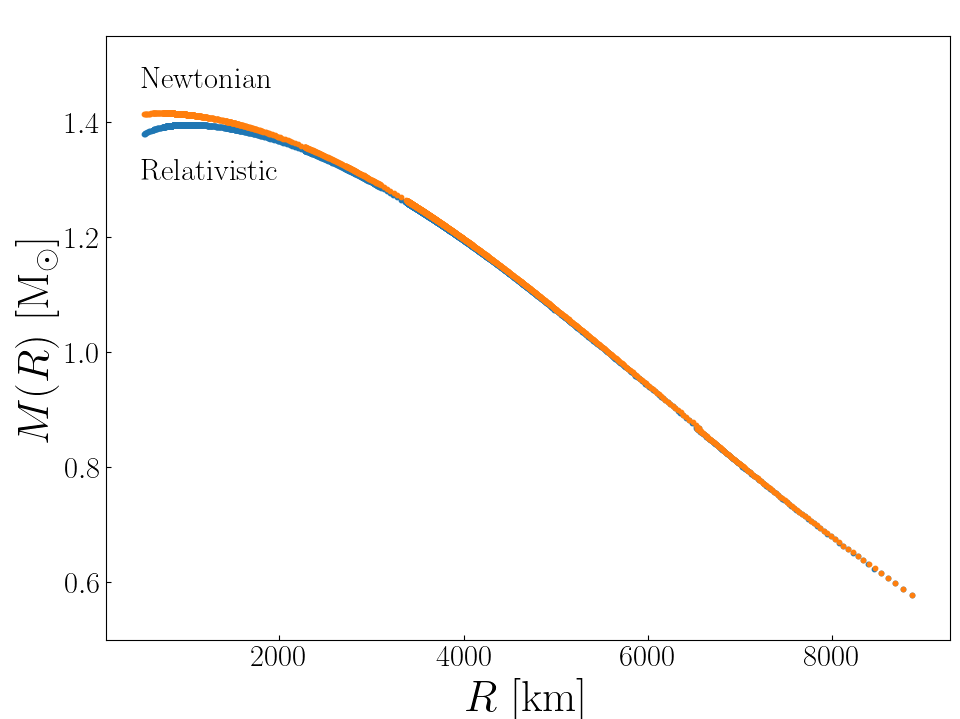
\includegraphics[scale=0.35]{WhiteDwarf_MR.png}
        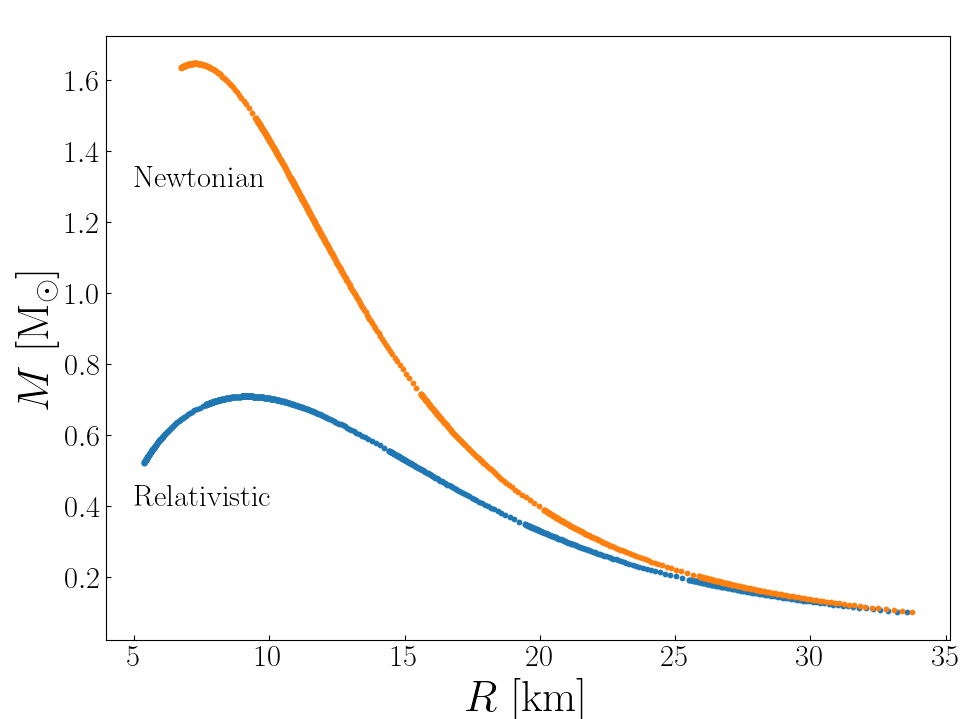
\includegraphics[scale=0.35]{Neutron_MR.png}
    \end{center}
    \caption{The mass-radius relationship for a white dwarf (top) and the mass as a function of pressure in the center of the star (bottom). The difference between the maximum mass between the newtonian and relativistic treatments is $0.02$ M$_\odot$.}
    \label{29maj0007}
\end{figure}
%\begin{figure}[t]
%    \begin{center}
%        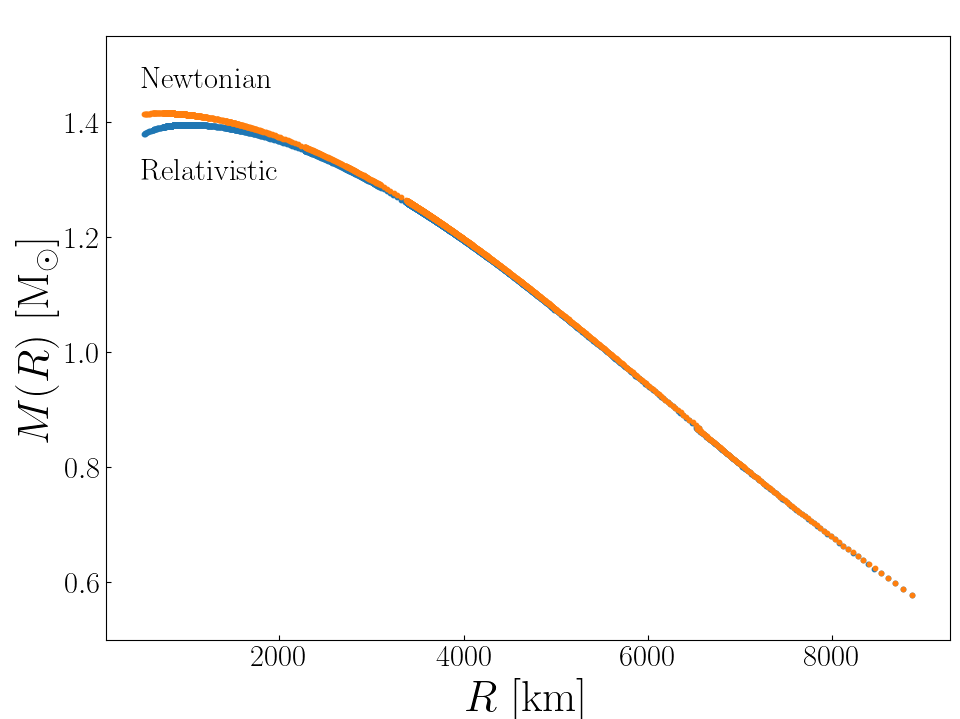
\includegraphics[scale=0.35]{WhiteDwarf_MR.png}
%        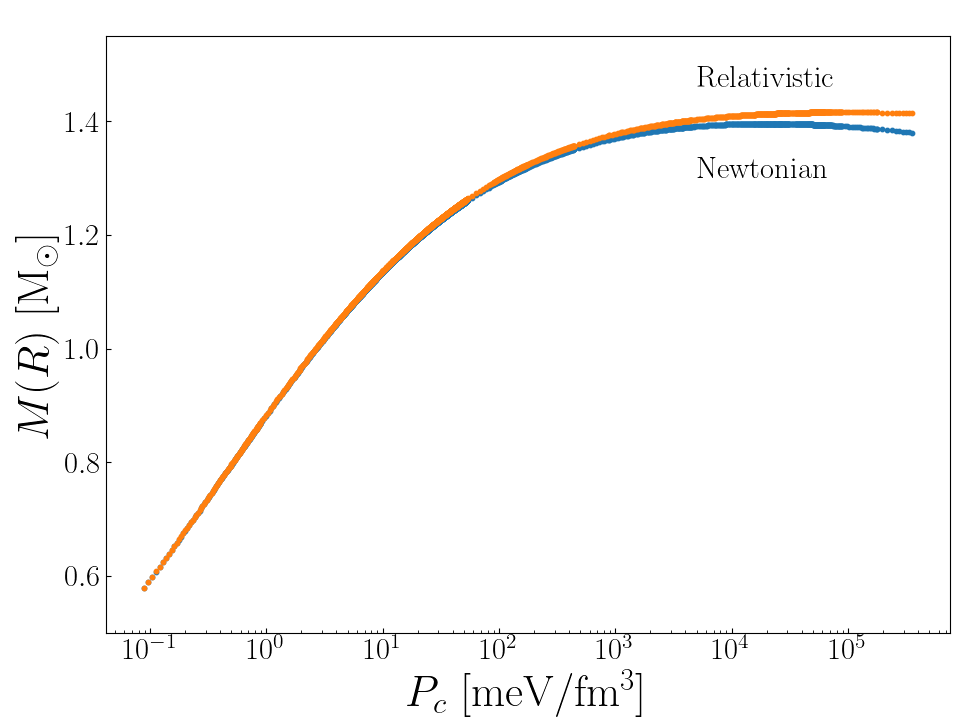
\includegraphics[scale=0.35]{WhiteDwarf_MP.png}
%    \end{center}
%    \caption{The mass-radius relationship for a white dwarf (top) and the mass as a function of pressure in the center of the star (bottom). The difference between the maximum mass between the newtonian and relativistic treatments is $0.02$ M$_\odot$.}
%    \label{29maj0007}
%\end{figure}
%\begin{figure}[b]
%    \begin{center}
%        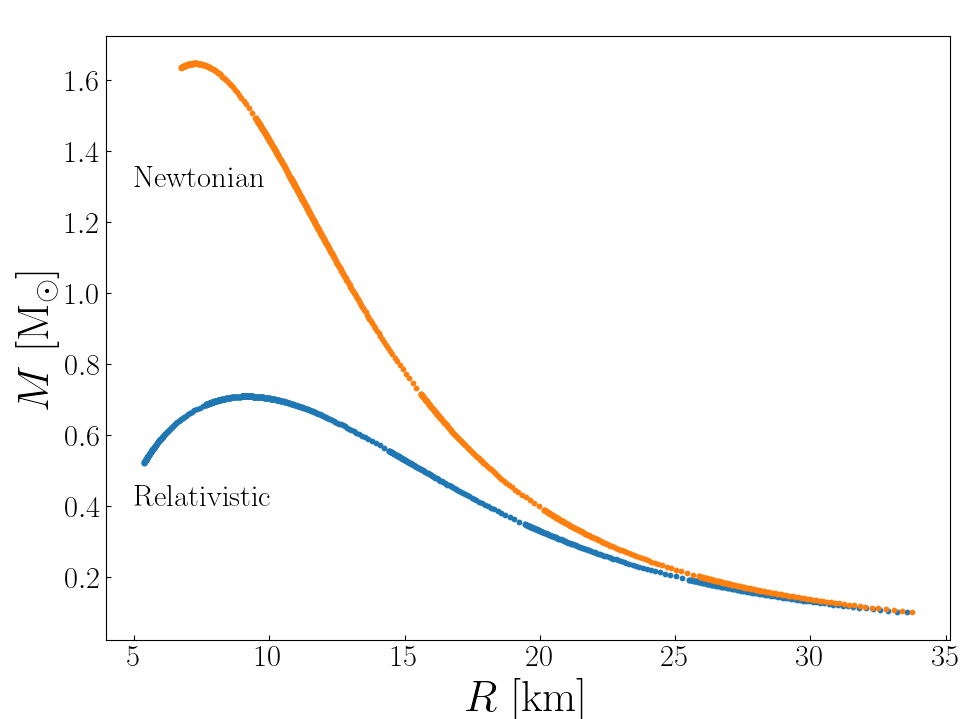
\includegraphics[scale=0.35]{Neutron_MR.png}
%        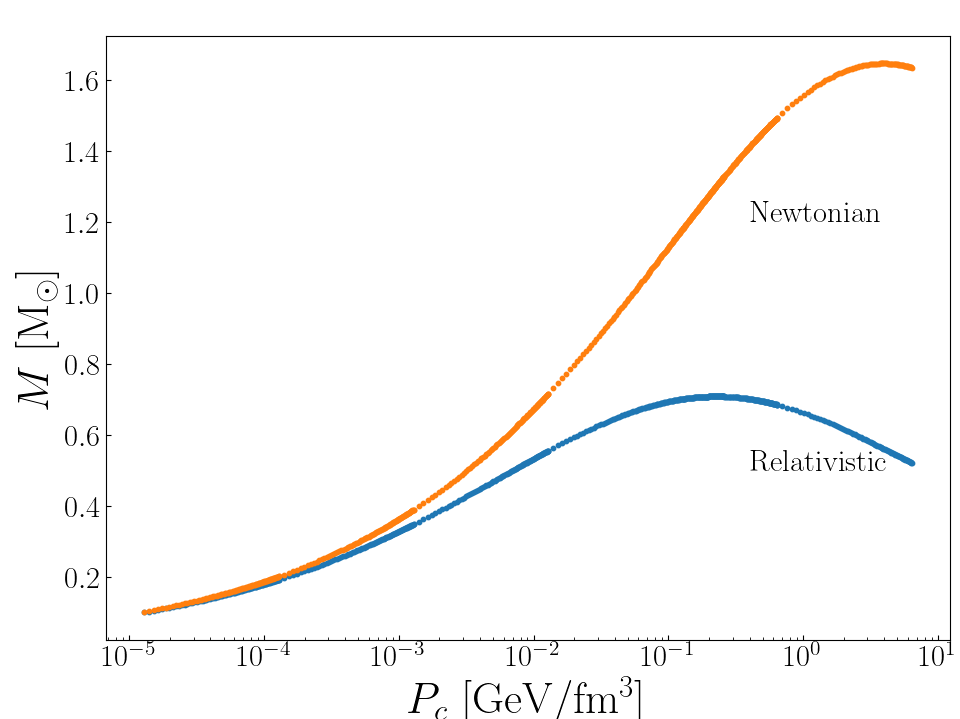
\includegraphics[scale=0.35]{Neutron_MP.png}
%    \end{center}
%    \caption{The mass-radius relationship for a neutron star (top) and the mass as a function of pressure in the center of the star (bottom). The difference between the maximum mass between the newtonian and relativistic treatments is $0.938$ M$_\odot$.}
%    \label{29maj0008}
%\end{figure}

%\begin{center}
%    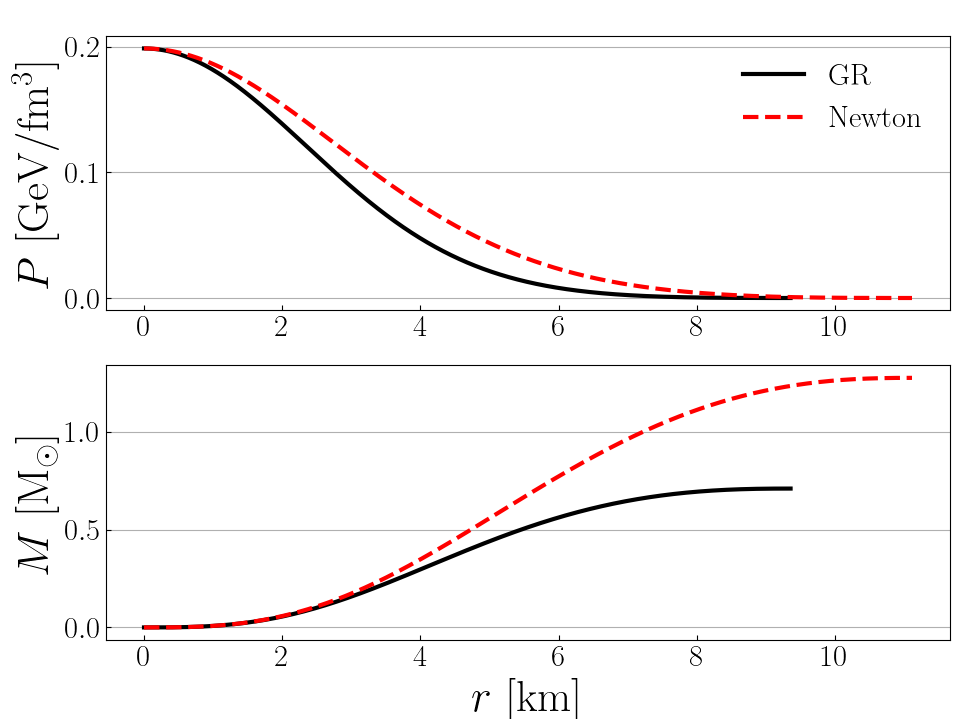
\includegraphics[scale=0.35]{Newt.png}
%\end{center}
%\begin{center}
%    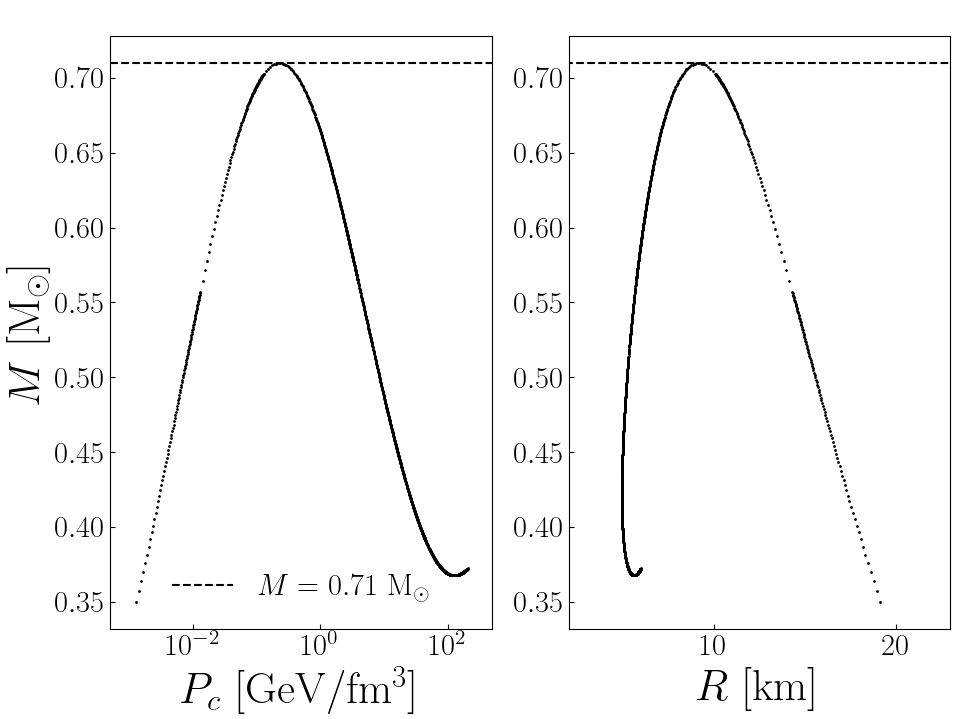
\includegraphics[scale=0.35]{TOV_limit.png}
%\end{center}



%\subsection*{Notes}
%\begin{itemize}
%    \item Compare with Newton  (x)
%    \item Also do white dwarfs (x)
%    \item Remove equation numberings which are not needed
%    \item Singular $x-2m$ term?
%    \item Do the series expansions?
%\end{itemize}




\end{large}
\end{document}
